%%%%%%%%%%%%%%%%%%%%%%%%%%%%%%%%%%%%%%%%%%%%%%%%%%%%%%%%%%%%%%%%%%%%%%%%%%%%%%%%%%%%
%Do not alter this block of commands.  If you're proficient at LaTeX, you may include additional packages, create macros, etc. immediately below this block of commands, but make sure to NOT alter the header, margin, and comment settings here. 
\documentclass[12pt]{article}
 \usepackage[margin=1in]{geometry} 
\usepackage{amsmath,amsthm,amssymb,amsfonts, enumitem, fancyhdr, color, hyperref,comment, graphicx, environ,mathtools, bbm, tikz, setspace, cleveref,listings, dcolumn}
\usepackage{array, multirow, caption, booktabs}
\usepackage{ mathrsfs }
\usetikzlibrary{matrix,positioning}
\tikzset{bullet/.style={circle,draw=black,inner sep=8pt}}
\DeclareMathOperator*{\argmax}{arg\,max}
\DeclareMathOperator*{\argmin}{arg\,min}
\DeclareMathOperator*{\Var}{\text{Var}}
\DeclareMathOperator*{\Cov}{\text{Cov}}

\DeclarePairedDelimiter\norm{\lVert}{\rVert}%
\newtheorem{theorem}{Theorem}
\newtheorem{lemma}[theorem]{Lemma}
\DeclareMathOperator{\eps}{\varepsilon}
\doublespacing
\DeclarePairedDelimiter\abs{\lvert}{\rvert}%
\pagestyle{fancy}
\setlength{\headheight}{65pt}
\newenvironment{problem}[2][Problem]{\begin{trivlist}
\item[\hskip \labelsep {\bfseries #1}\hskip \labelsep {\bfseries #2.}]}{\end{trivlist}}
\newenvironment{sol}
    {\emph{Solution:}
    }
    {
    \qed
    }


%%%%%%%%%%%%%%%%%%%%%%%%%%%%%%%%%%%%%%%%%%%%%%%%%%%%%%%%%%%%%%%%%%%%%%%%%%%%%%%%%


\usepackage{xcolor}
 
 


%%%%%%%%%%%%%%%%%%%%%%%%%%%%%%%%%%%%%%%%%%%%%

\rhead{Asha Bharadwaj, Caitlin Dutta, John Higgins, Alexis Smith\\Econ 899 \\ 19 October, 2022} 

%%%%%%%%%%%%%%%%%%%%%%%%%%%%%%%%%%%%%%%%%%%%%


%%%%%%%%%%%%%%%%%%%%%%%%%%%%%%%%%%%%%%

\begin{document}
\begin{table}[htbp]
    \centering
    \caption{Model moments for by $\alpha$, $c_F = 10$:}
      \begin{tabular}{lccc}
          \toprule
            Variable                & Standard             & $\alpha = 1$           & $\alpha = 2$           \\
          \midrule
            Price level                    & 0.739        & 0.691         &     0.720      \\
            Mass of Incumbents               & 7.385       & 8.756          & 7.625                 \\
            Mass of Entrants      & 1.778        & 2.685        & 2.257       \\
            Mass of Exits      & 0.6579          & 2.441           & 1.866                \\
            Aggregate Labor   & 171.336       & 178.582          & 173.505                   \\
            Labor of Incumbents   & 146.265          & 147.188          & 143.954               \\
            Labor of Entrants  & 25.071         & 31.394          & 29.551                  \\
            Fraction of Labor in Entrants   & 0.146         & 0.176         & 0.170                  \\
          \bottomrule
      \end{tabular}
    \label{tab:cf10}
  \end{table}
We list the model moments for each parameterization (non-stochastic, TIEV parameter $\alpha = 1$, and TIEV parameter $\alpha = 2$) in the above table. Recall that as the Type I Extreme Value distribution parameter $\alpha$ increases, the variance of the distribution decreases. Thus, higher $\alpha$ corresponds more closely to the non-stochastic case (where there is no uncertainty about the exit decision). We see this reflected in the above table. For $\alpha = 2$, the equilibrium outcomes are closer to the non-stochastic case, and are farther from the non-stochastic case for $\alpha = 1$. The price level is highest in the non-stochastic case and lower when $\alpha = 1$. Intuitively, low productivity firms may get a large $\epsilon$ shock which induces them to stay when it would have otherwise been optimal for them to exit. As a consequence, the exit behavior will be different from the non-stochastic specification. To fix ideas, consider the case where $\alpha = 1$: we observe that low-productivity firms only exit with probability roughly 52\%, meaning that around 48\% of low-productivity firms decide to stay (whereas they would have exited for sure in the deterministic case). Thus, the total mass of firms is higher than in the non-stochastic case, which leads to a lower price level (since there is more firms and thus more competition). To break down the difference by firm size, we plot the mass of firms of each size for each parameterization. We see that there are more low-productivity firms in the $\alpha = 1$ case than either of the other cases, which illustrates this point. As the variance of the TIEV distribution decreases, the exit behavior is closer to that of the non-stochastic case (and thus so are the equilibrium  outcomes).

\begin{center}
    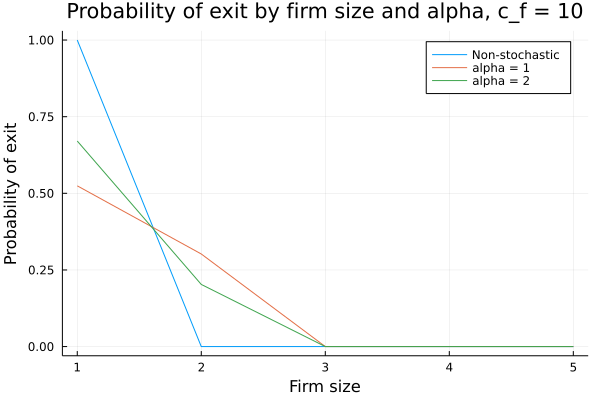
\includegraphics[scale=0.7]{exitplot10.png}
\end{center}

In the $\alpha = 1$ case, the mass of incumbents, entrants, and exits are all greater than the non-stochastic case. The reason is for the same logic above: there will be more low-productivity firms in steady state, and about half of them exit each period (versus all of them in the non-stochastic case). As a consequence, the steady state would require a higher mass of entrants to replace the exiting firms.

Aggregate labor is higher in the stochastic setting versus the non-stochastic setting, with aggregate labor under $\alpha = 1$ greater than labor under $\alpha = 2$. Similarly, the labor share of entrants is highest when $\alpha = 1$ (highest variance of TIEV), second highest when $\alpha = 2$ (lower variance of TIEV), and lowest in the non-stochastic case. This is explained as above by the higher mass of low-productivity firms for $\alpha = 1$. 

Plotted below is the exit probability by model specification. In the non-stochastic specification, the lowest-productivity firms will always exit and all other firms will remain in the market. This changes as we consider the stochastic specifications. As discussed above, the probability of exit for the smallest firms is lowest when $\alpha = 1$ (highest TIEV variance) and highest in the non-stochastic case. Again, the intuition for this is that the $\epsilon$ shocks cause some firms to stay in the market even when it would otherwise be profitable for them to exit. We see that firms of size 2 (i.e. those with productivity 3.58 ) have higher exit probability under $\alpha = 1$ than both $\alpha = 2$ and the non-stochastic specification. Intuitively, there are too many of the smallest firms, which means that in steady state we must have higher rate of exit from the next highest firm size (in order to have an invariant distribution). 

As the variance of the TIEV shocks decreases (i.e. $\alpha$ goes from 1 to 2), firm behavior becomes closer to the non-stochastic specification. We see that the exit probability for $\alpha = 2$ (low TIEV variance) is essentially a convex combination of the exit probability of $\alpha = 1$ (high TIEV variance) and the non-stochastic case (no variance). 

For fun (loosely interpreted), we also plot the invariant distribution of firm sizes by model specification. When $\alpha =1$, there is a higher mass of the smallest firms than in the non-stochastic case and $\alpha = 2$. To balance it out, there are less size 2 firms for $\alpha = 1$. There are also more size 3-5 firms under $\alpha = 1$ than the other specifications. 
\begin{center}
    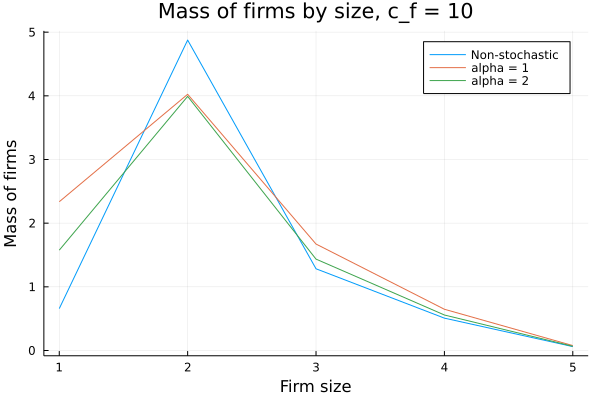
\includegraphics[scale=0.7]{muplot10.png}
\end{center}
We now consider what happens when $c_f$ increases to 15. We provide a similar table under this specification:
\begin{table}[htbp]
    \centering
    \caption{Model moments by $\alpha$, $c_F = 15$:}
      \begin{tabular}{lccc}
          \toprule
            Variable                & Standard             & $\alpha = 1$           & $\alpha = 2$           \\
          \midrule
            Price level                    & 0.889      & 0.862        &     0.825      \\
            Mass of Incumbents               & 2.643      & 3.651          & 3.447                \\
            Mass of Entrants      & 1.865        & 1.812       & 2.375      \\
            Mass of Exits      & 1.554         & 1.565           & 1.988                \\
            Aggregate Labor  & 166.479       & 173.188          & 174.129                  \\
            Labor of Incumbents   & 122.533         & 134.042         & 128.610                \\
            Labor of Entrants  & 43.945        & 39.146         & 45.518                  \\
            Fraction of Labor in Entrants   & 0.264         & 0.226         & 0.261                  \\
          \bottomrule
      \end{tabular}
    \label{tab:cf15}
  \end{table}
We also plot the exit decision rule and the invariant distribution of firms for each model specification given $c_f = 15$ below:
\begin{center}
    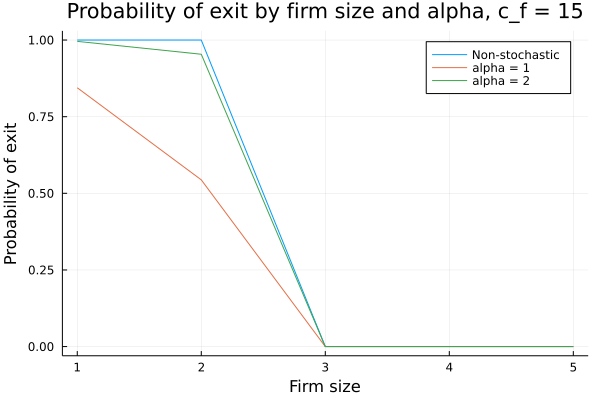
\includegraphics[scale=0.7]{exitplot15.png}
\end{center}
Here, we see that exit probabilities are higher than when $c_f = 10$. This makes sense: when the fixed cost to be paid to stay in the market is higher, the marginal firm under $c_f = 10$ will exit when $c_f = 15$. As before, we observe that the exit probability is lower when $\alpha = 1$ (i.e. higher variance of the TIEV shocks) than it is when $\alpha = 2$ (lower TIEV shock variance). Furthermore, the exit probabilities for both $\alpha=1$ and $\alpha = 2$ are lower than in the non-stochastic specification. 

We also plot the mass of firms by size when $c_f = 15$ below:
\begin{center}
    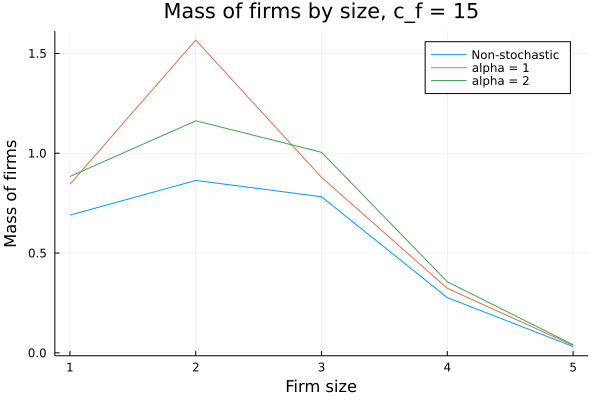
\includegraphics[scale=0.7]{muplot15.png}
\end{center}
\end{document}
